\section{Optics Measurements}



% ===============================
%           TbT Data
% ===============================
\subsection{\review{Turn-by-Turn Data}}

Data is typically acquired turn by turn while exciting the beam with an AC-Dipole. This is usually
done with a \textit{pilot bunch}, with a reduced intensity of $10^{11}$ protons compared to
an operation bunch of $10^{12}$. This allow for higher amplitude oscillations while remaining safe 
for the machine. \todo{intensity?} 

A spectral analysis is then performed via a \textit{FFT}, making apparent the driven tunes from the 
AC-Dipole, the transverse tunes and the possible resonance lines, as shown in
\cref{fig:optics_measurements:tbt_data:spectrum}.

\begin{figure}[H]
    \centering
    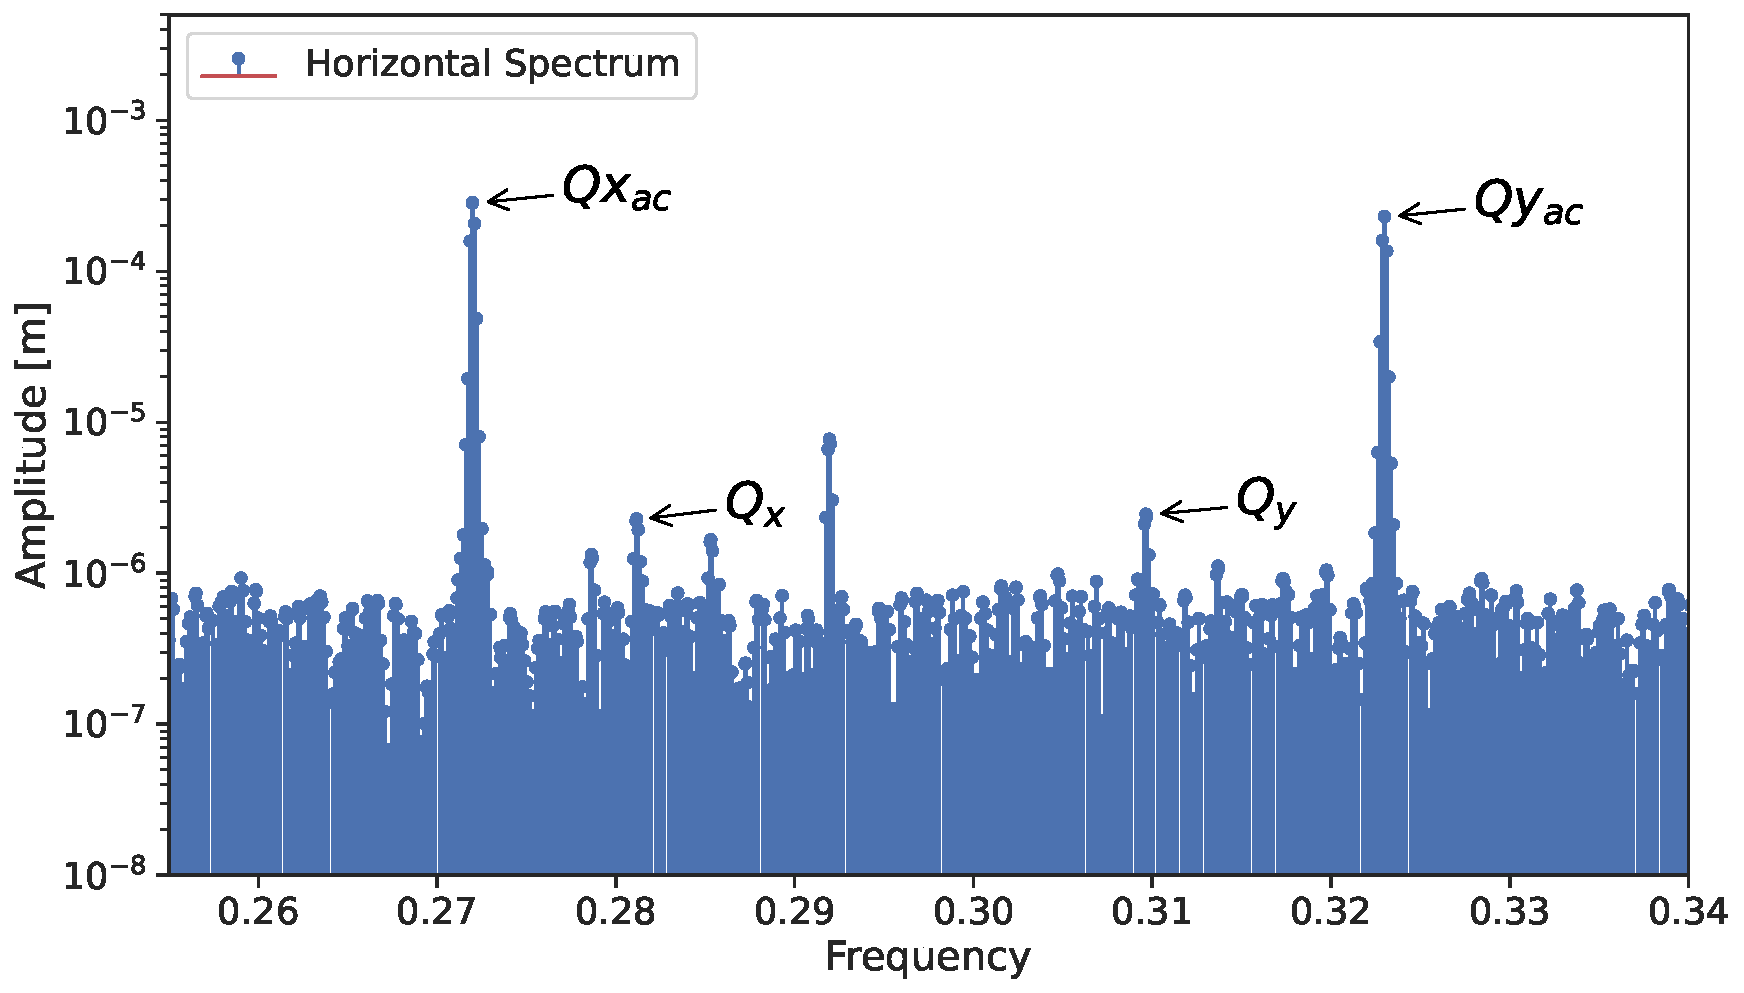
\includegraphics[width=0.8\textwidth]{./images/basic_spectrum.pdf}
    \caption{Horizontal frequency spectrum of a turn-by-turn measurement in the LHC. The 
    \textit{driven} tunes of the AC-Dipoles have the highest amplitudes while the natural tune can
    be seen close to it. Other lines are often created by resonances.}
    \label{fig:optics_measurements:tbt_data:spectrum}
\end{figure}

From this, the \textit{optics} such as $\beta$-beating, dispersion, coupling and Resonance Driving
Terms can be reconstructed~\cite{catalan-lasheras_linear_2004}.



% ===============================
%         Chromaticity
% ===============================
\subsection{\review{Chromaticity}}
\label{subsection:optics_corrections_chromaticity}

% --- Procedure ---
\subsubsection{\review{Procedure}}

Chromaticity measurements are typically performed by varying the RF frequency to induce a change of
momentum offset $\delta$, while measuring the tune.  The momentum offset $\delta$ being related to
the RF frequency, the Lorentz factor $\gamma$ and the momentum compaction factor
$\alpha_c$~\cite{keintzel_jacqueline_beam_nodate}:

\begin{equation}
    \delta = - \left(\frac{1}{\gamma^{-2} + \alpha_c}\right) \cdot \frac{\Delta f_{\text{RF}}}{f_{\text{RF,nominal}}}
    \label{eq:dpp_rf}
\end{equation}

In the LHC, the Lorentz factor $\gamma$ is here negligible, as the energy is large even at injection.
At 450GeV, $\gamma^{-2} \approx 10^{-6}$, which is two orders of magnitude smaller than $\alpha_c$.

Frequency steps of 20Hz every 30 secondes are usually taken to compromise between number of data
points, precision of the tune estimate, and duration of the measurement. Once beam losses,
registered by the BLMs are deemed too high, the frequency is reverted back to its nominal value in
larger steps. The same procedure is then re-applied in the negative. Figure
\ref{fig:measurements:rf_scan} shows a typical RF scan performed to measure chromaticity in the LHC.

\begin{figure}[H]
    \centering
    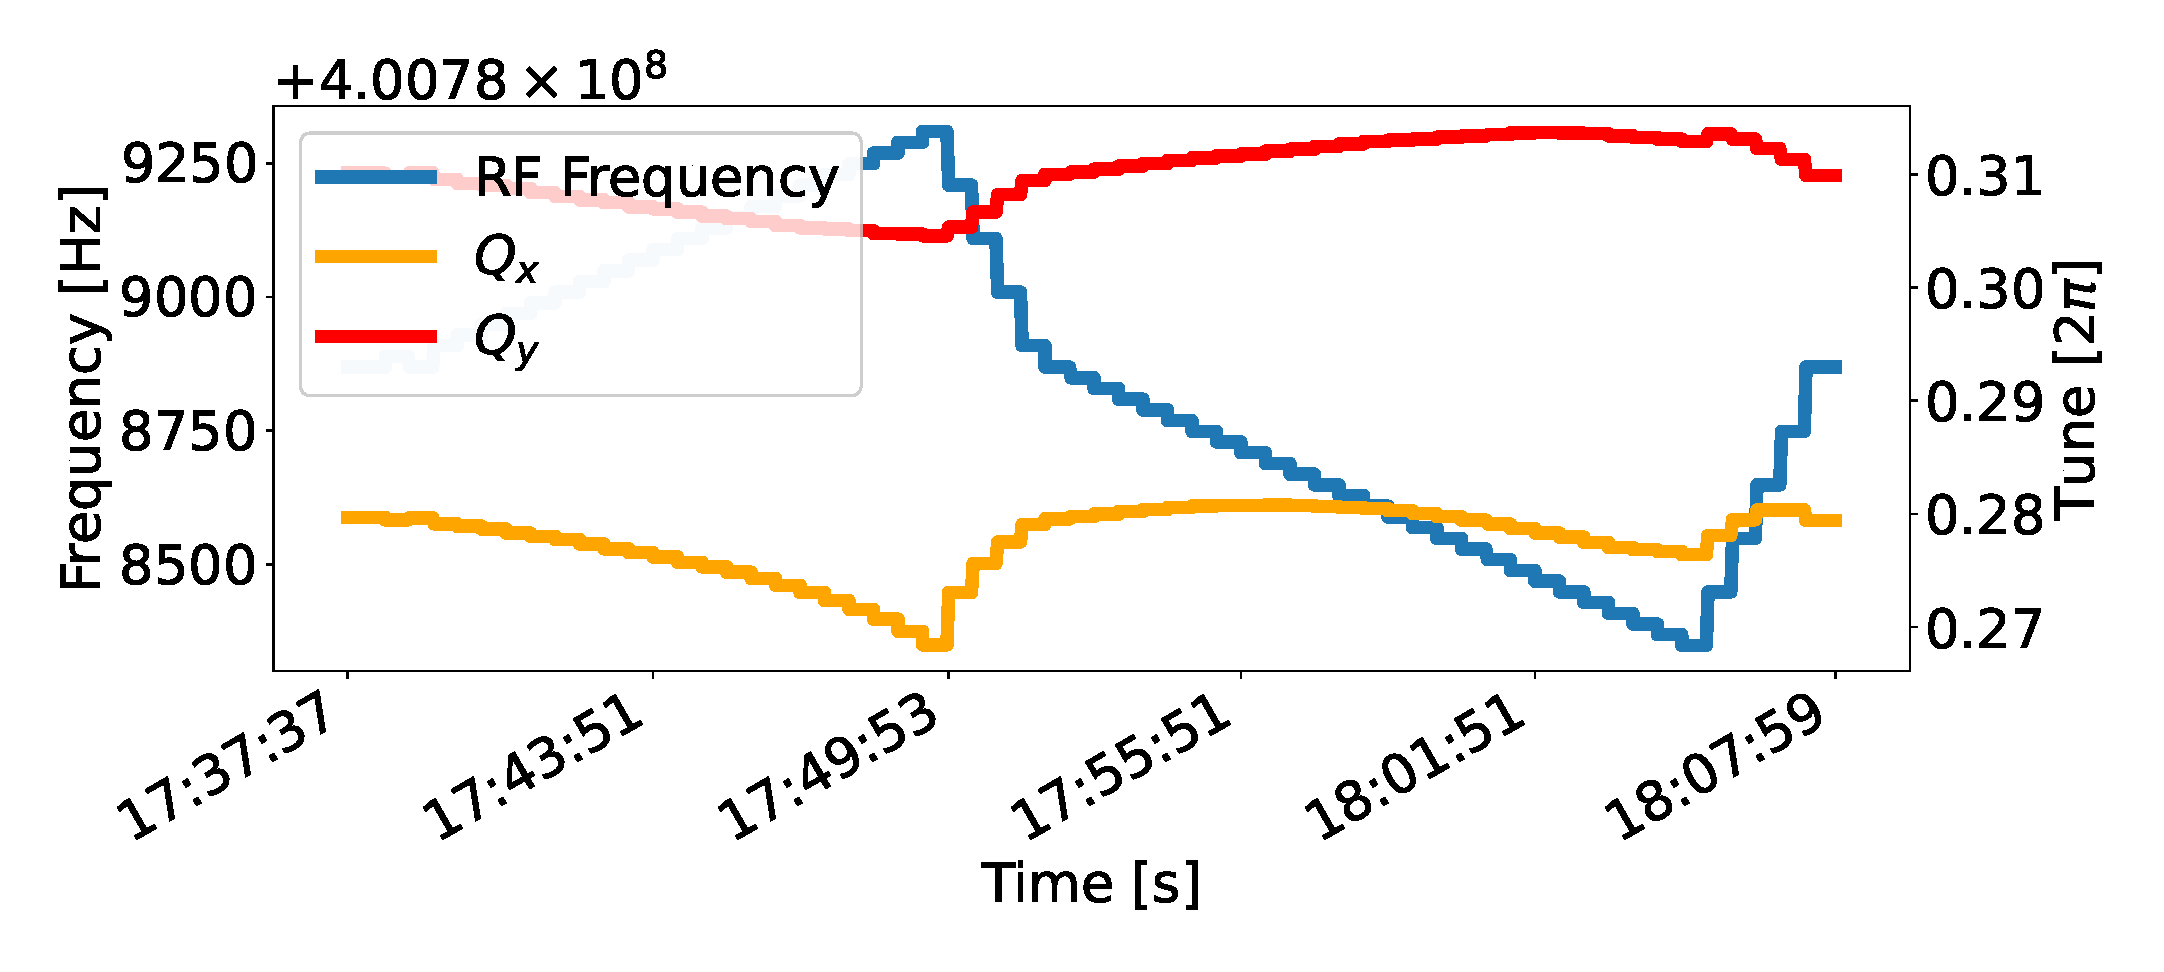
\includegraphics[width=1\textwidth]{images/rf_scan.pdf}
    \caption{Observation of the tune dependence on momentum offset, created by a shift of RF
             frequency.}
    \label{fig:measurements:rf_scan}
\end{figure}




% --- Analysis and Fit ---
\subsubsection{\review{Analysis}}

Once the tunes have been acquired and the momentum offset computed via \cref{eq:dpp_rf}, the
chromaticity function (see \cref{eq:background_chromaticity}) can be used to fit the
measured data and retrieve each order.

As part of work for this thesis, a custom tool was developed, in order to ease such analysis of
chromaticity measurements. This tool, the Non-Linear Chromaticity
GUI~\cite{m_le_garrec_non-linear_2022}, is composed of several parts:

\begin{itemize}
    \tightlist
    \item Data extraction from CERN data servers (Timber, NXCALS)
    \item Tune cleaning and standard deviation calculation
    \item Chromaticity fit up to 7th order
    \item Corrections of chromaticity and resonance driving terms
\end{itemize}

%\todo{if the screenshot actually useful?}
%
%Fits up to the third and fifth order using this tool can be seen in Fig.\ref{fig:chroma_gui}.
%
%\begin{figure}[H]
%    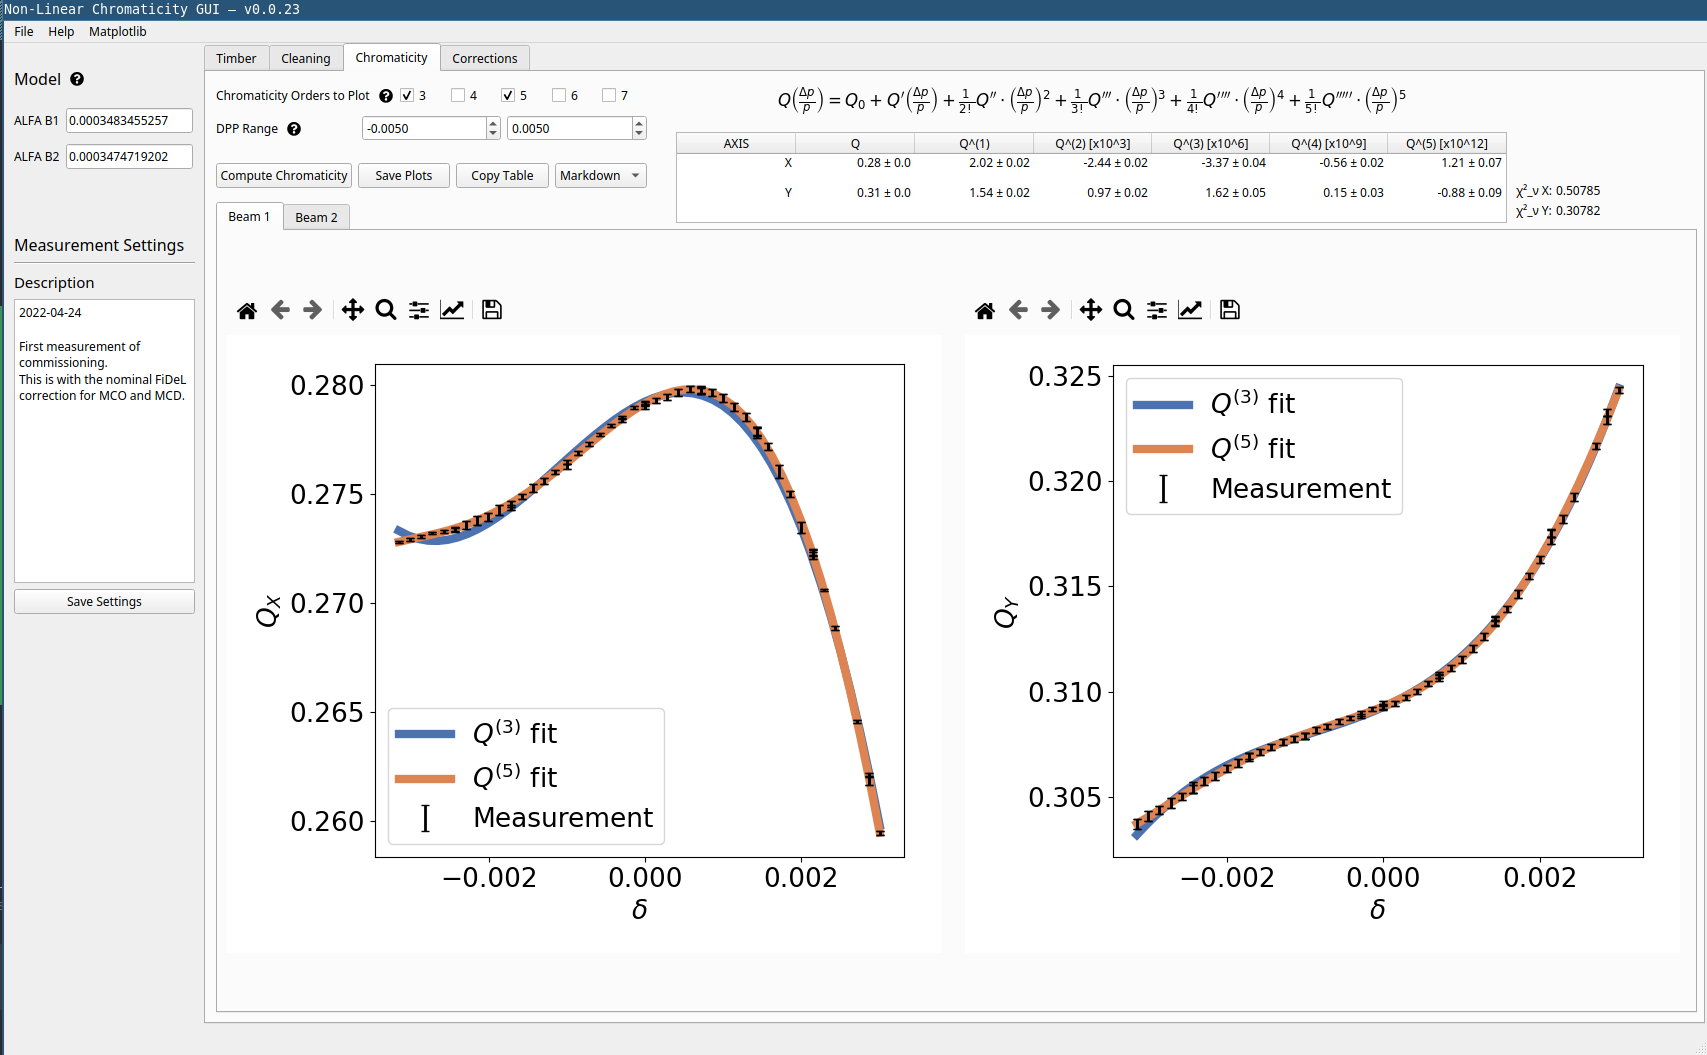
\includegraphics[width=\textwidth]{./images/chroma_gui.png}
%    \caption{\textit{Non-Linear Chromaticity GUI} program, used to automatize chromaticity 
%             analysis.}
%    \label{fig:chroma_gui}
%\end{figure}